\providecommand{\main}{./report}
\documentclass[../main.tex]{subfiles}
\begin{document}


\section{Motivations}\label{section:motivations}


\subsection{Motivations for Feature Ranking}
% motivation for ranking and weighting features:
The desire to create a feature ranking from some features in a dataset stems from two main applications: the domain of feature selection and the domain of interpretable AI. To better understand why one would want to create a feature ranking, a brief exploration is made on both domains, motivating the concept throughout.



% (1) feature selection
\subsubsection{Feature Selection}
% cure of dimensionality
The field of Machine Learning is plagued by the curse of dimensionality \citep{koppen_curse_2009}: as the dimensionality of datasets grows larger, the computational burden for learning algorithms gets exponentially larger. This is due to the fact that when data gets of increasingly higher dimensionality, the volume of the data shape grows faster than the amount of samples grows along, causing the data volume to become sparse.
% biomedical world example
There are many real-world domains that naturally deal with datasets of such shape. In the biomedical world, for example, collecting data samples might require arduous amounts of human effort \citep{hu_feature_2018}. There might be the case where one data sample represents one human and any such sample is very laborious to collect: but the samples that are collected are of very high dimensionality. In this case, we deal with a scenario where the amount of dimensions far exceeds the amount of samples ($n \gg p$ where $n$ is the amount of samples and $p$ the amount of dimensions).

% avoid curse of dimensionality using feature selection
To avoid such a curse of dimensionality, feature selection can be used. The goal is to reduce as much features as possible while retaining the most relevant information in the dataset. The benefits are a decreased computational burden; though in some cases the learning algorithm generalization performance might actually be improved over a scenario when no feature selection is used. This is most often due to the removal of noise that would have interfered with the learning process.

% example: feature ranking to feature selection
One such example process of feature selection by using a feature ranking can be seen in Figure~\ref{fig:schematic-feature-selection}. As can be seen in the figure, a ranking can be used to reduce the overall dataset size by using a \textit{threshold} operation. In such a threshold operation, any feature that ranks below the given threshold $\epsilon$ is removed. Many, if not most, feature selection methods rely on feature ranking methods under the hood to create a feature subset of reduced size.

\begin{figure}[h]
    \centering
    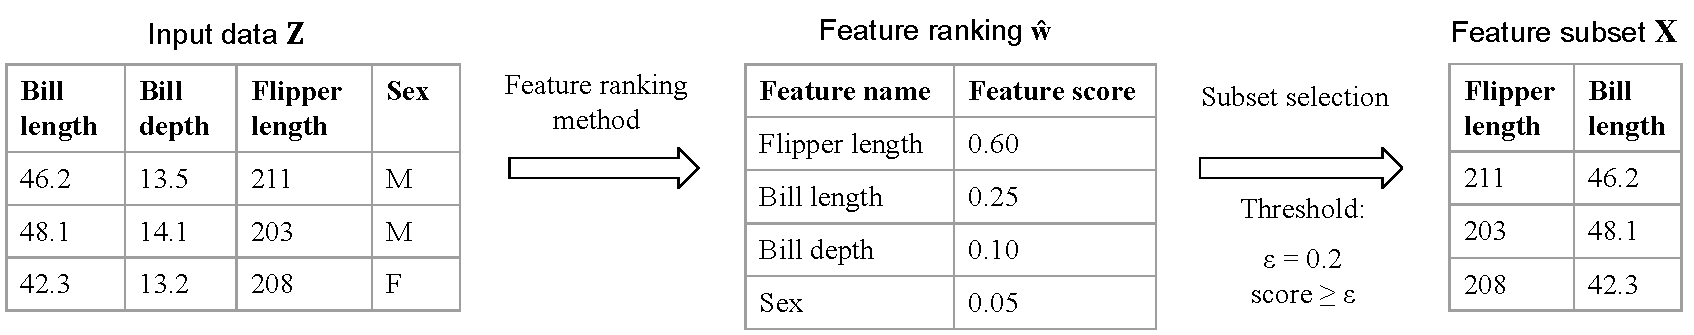
\includegraphics[width=\linewidth]{report/images/schematic-feature-selection.pdf}
    \caption{An example process of feature selection by thresholding a feature ranking at some point $\epsilon$. The resulting feature subset $\mathbf{X}$ presumably contains the strongest predictors given the target variable. Feature names come from a real dataset on antarctic penguins \citep{horst_palmerpenguins_2020}.}
    \label{fig:schematic-feature-selection}
\end{figure}

% so: feature ranking is important for feature selection -> they go hand in hand
For this reason, the more general problem of constructing feature rankings is omni-relevant in the feature selection domain. To go from feature ranking to feature selection, the only extra step necessary is a sufficient threshold point, which many algorithms arrive at using different methods. A straightforward way to cut off low-ranking features is to exclude any feature that ranks below the mean score - or, alternatively, exclude only the highest ranking quartile, etcetera. More sophisticated schemes exist, however. One might also choose to iteratively run a feature ranking process and remove the lowest ranking score in each iteration. Such a process is called \gls{rfe}. That said, it is clear that feature ranking and feature selection go in unison.





% (2) interpretable AI
\subsubsection{Interpretable Artificial Intelligence}
% algorithms became harder to reason about
The domain of Interpretable AI has arisen due to the need to better understand and reason about the decisions that any Machine Learning model makes. Traditionally, the sole goal in building a learning algorithm would be to best predict some target variable, given some set of samples to learn from. With the advent of sophisticated learning algorithms such as Neural Networks and especially Deep Neural Networks, however, the many computational layers that separate inputs from answers tend to obfuscate the decision process \citep{rai_explainable_2020}. Whereas in classical statistical models practitioners sought to unveil a clear relationship between the independent- and dependent variables, some models in the field of Machine Learning have grown so complicated that no human can reason on its output. Because such algorithms tend to compare metaphorically to a black box one cannot possibly see through, one also refers to such algorithms as \textit{black boxes}.

% ML is used in professional world: we need transparency
Whilst at the same time models have gotten progressively more sophisticated and thus less transparent, the market for deploying Machine Learning has been steadily getting bigger. Many institutions seek to benefit from the possibilities of recent developments in \gls{ai} and \gls{ml} - including many companies, schools or the government. In all such applications, for every decision made by a Machine Learning model, an argumentation as how the model came to such a conclusion is desired. Even, in some scenarios the decision to be made at hand weighs so heavily that a \gls{ml} model that cannot explain itself might not be usable at all. For example, one might deploy a \gls{ml} model that scores employees based on their performance. The goal is then to fire the lowest ranking employees and keep highest performing ones. But fully trusting such a model might be a dangerous practice. If a model provides only bare explanations on how it came to such a decision, employers might have a hard time interpreting the model and employees might have a hard time understanding its decisions. As a matter of fact, faulty models of such kind have already been deployed out in the open - with considerable complications with respect to model transparency as a result \citep{oneil_weapons_2016}.

% interpretable AI to the rescue (two ways: (1) make model less complicated, (2) explain model)
For this reason, decisions made by computers are required to be explainable - allowing practitioners to assess not only \gls{ml} model decisions, but also assess the overall usefulness of the model in general. After all, many learning models are designed such to always generate a decision, no matter how noisy the input. That said, the black box of AI can generally be opened up in two ways. First, one could opt for a less sophisticated in the first place - one that reveals its inner workings and supports its decisions by an elaborate scheme, much in line with classical statistics. Although a simpler model could sometimes suffice in places where practitioners currently opt for more complicated ones, a solution for models of any kind of flexibility is desired. Therefore, a second option is to delve into any such model to reveal a reasoning about its decision-making process - which is the option that the field of Interpretable AI bothers itself with.

% feature rankings in interpretable AI
Feature rankings are one of the facets which can be used to facilitate a better understanding of a Machine Learning model \citep{hansen_interpretability_2019}: by unveiling which variables the \gls{ml} model finds important, a better understanding can be gained on its decision-making process. In some scenarios, it might, for example, be the case that the Machine Learning model in question unexpectedly weighs a feature as very important, even though a human expert can know apriori that the feature is not of value to the predictive task at hand. In this way, faulty models can be detected and prevented from being used in critical settings. In the Interpretable AI jargon, the process of scoring and explaining feature importance goes under different names. In the literature, feature rankings are referred to as \textit{feature impact} scores, \textit{feature importance} scores, or \textit{feature effects}, which are synonymous in this case. All terms indicate the process of quantifying feature relevance with respect to the learning task at hand. The general process of an interpretable AI algorithm can be seen as in Figure~\ref{fig:schematic-interpretable-ai}.

\begin{figure}[ht]
    \centering
    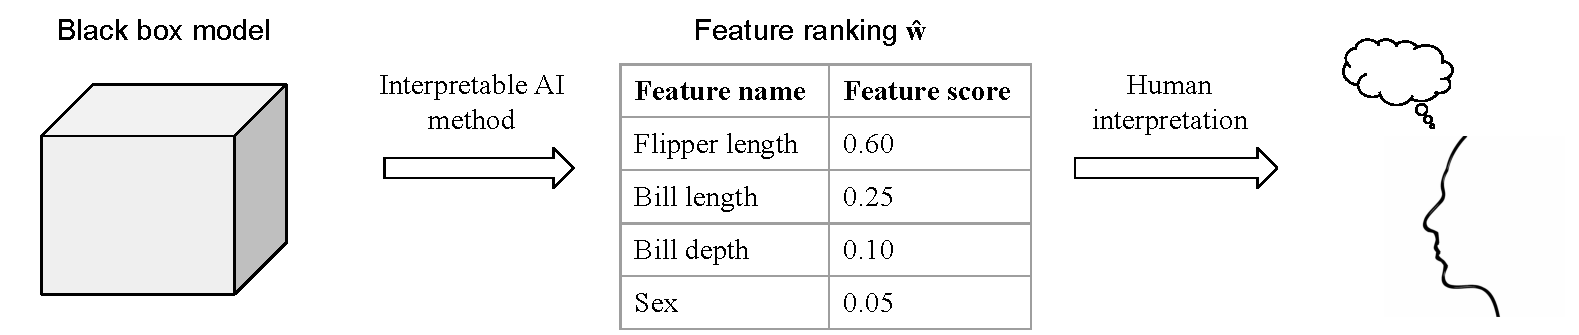
\includegraphics[width=\linewidth]{report/images/schematic-interpretable-ai.pdf}
    \caption{An example process of Interpretable AI. In this case, the input to the interpretable AI algorithm is a trained black box model, which has an otherwise hard to understand decision making process. The interpretable AI algorithm then extracts feature importance scores for better interpretability.}
    \label{fig:schematic-interpretable-ai}
\end{figure}

% so: feature rankings are important for interpretable AI.
As could be seen in Figure~\ref{fig:schematic-interpretable-ai}, one way of making a black box model more interpretable is to extract a feature ranking from the trained model - an interpretable AI algorithm reads in the black box model and tries to explain it \citep{lundberg_unified_2017}. Other interpretable AI methods take a more direct approach \citep{arik_tabnet_2020}, in which the interpretable AI algorithm functions as a prediction method itself. The latter approach is employed only in more recent years; in which learning algorithms are designed from the start to be interpretable. However, independent of whether a direct- or indirect approach to explaining the decision process is taken, the desire to rank features is applicable to both. That said, we can therefore conclude that the construction of truthful feature rankings are an important aspect in interpretable AI.




\subsection{Motivations for Evaluating Feature Ranking methods}
Given the need for Feature Ranking methods, the desire to evaluate such methods systematically is clear. Practitioners throughout the field of Machine Learning desire to know the behavior of different methods under a large range of varying conditions, such as the sample size-, dimensionality-, or domain of the dataset. One also needs to take into account the available computational resources and the desired degree of accuracy of the solution. Finding out what evaluation methods and metrics best represent the optimality of the solution is essential, for else the presentation of scientific findings might be misleading compared to real-world performance.

In this way, individuals and institutions are motivated to actively research Feature Ranking methods and evaluate them such to determine which method works best, under what conditions. As is more often the case in the comparison of Machine Learning algorithms, however, is the fact that methods are not always easily analytically compared. That is, solely a theoretical analysis does not suffice to create a meaningful comparison. Although one can reason about the performance of many methods before conducting concrete data analyses, a real-world experiment is essential to any reputable publication.



\biblio
\end{document}